\documentclass{article}
% translate with >> pdflatex -shell-escape <file>

\usepackage{pgfplots}
\pgfplotsset{compat=newest}

\pagestyle{empty}

\begin{document}
\begin{tikzpicture}[scale=1]%
  \begin{axis}[
      width=0.8\textwidth,
      height=0.6\textheight,
      title=Plot of factorial,
      ylabel style={overlay},
      yticklabel style={overlay},
      xlabel={$x$},
      ylabel={$y$},
      %legend style={at={(0.5,0.97)},mark=none,
      %   anchor=north,legend columns=-1},
      legend style={ overlay, at={(-0.3,.5)}, anchor=center}, every axis plot post/.append style={mark=none},
      domain=2:10,
      ymax=43000
   ]
    \addplot[mark=x] coordinates {
      (0, 1)
      (1, 1)
      (2, 2)
      (3, 6)
      (4, 24)
      (5, 120)
      (6, 720)
      (7, 5040)
      (8, 40320)
    };
    
   \legend{$x!$}
   \end{axis}
\end{tikzpicture}%
\end{document}
